\section{Simulationen zur Steuerung von Quadrokoptern}
Die Popularität von Unbemannten Flugzeugen im letzten Jahrzehnt nahm besonders im Bereich der Quadrokopter zu, sodass zahlreiche zukunftsträchtige Ergebnisse und Anwendungen erforscht worden sind durch die sinkenden Kosten von Sensorik und Minicomputern. \footcite[Vgl.][S. 1]{Koch.2018}
Anwendungsfälle beinhalten z.B. die Landwirtschaft, den Pakettransport oder die Überwachung von großflächiger Infrastruktur wie Stromnetze. \footcite[Vgl.][S. 1]{Deshpande.2020}

\subsection{Flugdynamiken eines Quadrokopters}
Die Simulation des Quadrokopters stellt eine Simulation eines Flugkörpers mit drei Rotations- und drei Translationsbewegungen und demnach insgesamt sechs verschiedenen Freiheitsgraden dar. \footcite[Vgl.][S. 2]{Koch.2018}
Ein Quadrokopter ist dabei ein fester Körper mit vier befestigten Rotoren welche sich ausschließlich in eine Richtung drehen und positiven Schub in die Z-Achse des Körpers ausüben können. \footcite[Vgl.][S. 3]{Molchanov.2019}
Die vier Rotoren werden als + oder X Konfiguration entweder direkt in Richtung der X- und Y-Achse (+), oder um 45° gedreht (X) an der Drohne befestigt. \footcite[Vgl.][S. 2]{Koch.2018}
Jede Bewegung der sechs verschiedenen Arten wird durch die unterschiedliche Steuerung, der im Fall des Quadrokopters, vier Rotoren getätigt.
Eine unterschiedliche Ansteuerung der Rotoren und den demnach verschieden starken Auftrieben resultiert in den drei Rotationsbewegungen Rollen, Nicken und Gieren. \footcite[Vgl.][S. 2]{Koch.2018}
\begin{figure}[htb]
    \centering
    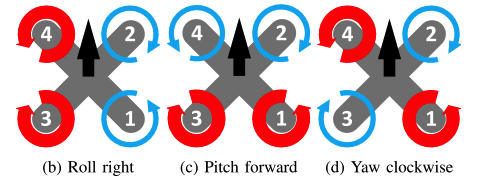
\includegraphics[height=3cm]{lib/graphics/Drone axis.png}
    \caption[Rotationsbewegungen eines Quadrokopters]{Rotationsbewegungen eines Quadrokopters\footnotemark}
    \label{abb:drone axis}
\end{figure}
\footnotetext{Enthalten in: \cite[][S. 2]{Koch.2018}}

Rollen wird wie aus Abbildung drei hervorgeht durch unterschiedlichen Auftrieb der zwei linken oder rechten Rotatoren, das Nicken durch Unterschiede der vorderen und hinteren Rotatoren hervorgerufen.
Das Gieren bzw. die Rotation um die Z-achse wird durch die stärkere Rotation der sich im Uhrzeiger drehenden oder der sich gegen den Uhrzeiger drehenden Rotoren bewerkstelligt. 

Diese Rotationsbewegungen werden mathematisch repräsentiert als Matrix der Eulerschen Winkel, welche die Folge der einzelnen Drehungen entlang der X-, Y-, und Z-Achse enthält. \footcite[Vgl.][S. 3]{Deshpande.2020}
Das Zusammenspiel dieser Rotationsbewegungen, dargestellt anhand Formel vier, mit der durch die Rotatoren entlang der Z-Achse der Drone erzeugte Schubkraft und den Rollraten, beschrieben in Formel fünf, sorgt für die Bewegung der Drohne in Richtung der zukünftigen Koordinaten nach Formel sechs. \footcite[Vgl.][S. 2]{Deshpande.2021}

\begin{description}
    \item \begin{center} (4) $R = \begin{pmatrix} C_{\psi}C_{p} & S_{\xi}S_{p}C_{\psi} - S_{\psi}C_{\xi} & S_{\xi}S_{\psi}+S_{p}C_{\xi}C_{\psi} \\ S_{\psi}C_{p} & S_{\xi}S_{\psi}S_{p} + C_{\xi}C_{\psi} &  -S_{\xi}C_{\psi} + S_{\psi}S_{p}C_{\xi}\\ -S_{p} & S_{\xi}C_{p} & C_{\xi}C_{p} \end{pmatrix}$ \end{center}
\end{description}
In Formel vier wird der Rotationszustand der Drohne zur den Weltachsen durch die Sinus- und Cosinuswinkel $S_{a}$ und $C_{a}$ repräsentiert, wobei für $a$ die Art der Rotation also Rollen $(\xi)$, Nicken $(p)$ und Gieren $(\psi)$ eingesetzt wird. \footcite[Vgl.][S. 2]{Deshpande.2021}
\begin{description}
    \item \begin{center} (5) $I\begin{pmatrix} \dot p \\ \dot q \\ \dot r\end{pmatrix} = \begin{pmatrix} l(F_{1} + F_{2} - F_{3} - F_{4}) \\ l(-F_{1} + F_{2} + F_{3} - F_{4}) \\ -M_{1} + M_{2} - M_{3} + M_{4}\end{pmatrix} - \begin{pmatrix} p \\ q \\ r \end{pmatrix} \times I\begin{pmatrix} p \\ q \\ r \end{pmatrix}$ \end{center}
\end{description}
Formel fünf inkludiert in der Matrix $I$ die Trägheitsmomente um die X-, Y- und Z-Achsen in Abhängigkeit der Rollrate $p$, Nickrate $q$ und Gierrate $r$. \footcite[Vgl.][S. 2]{Deshpande.2021}
Der Schub, der in der Länge $l$ vom Schwerpunkt entfernten Rotatoren, wird mittels $F_{i}$, das Drehmoment mit $M_{i}, \forall i \in \{1,2,3,4\}$ gekennzeichnet. \footcite[Vgl.][S. 3]{Deshpande.2020}
\begin{description}
    \item \begin{center} (6) $m\begin{pmatrix} \ddot x \\ \ddot y \\ \ddot z \end{pmatrix} = \begin{pmatrix}0 \\ 0 \\ -mg\end{pmatrix} + R\begin{pmatrix} 0 \\ 0 \\ \sum_{i=1}^{4} F_{i} \end{pmatrix}$ \end{center}
\end{description}
Weiterhin ist die Beschleunigung in Richtung der Koordinaten $\ddot x$, $\ddot y$ und $\ddot z$ durch die die Masse $m$ und der Gravitation $g$ beeinflusst. \footcite[Vgl.][S. 3]{Deshpande.2020}

\subsection{Repräsentation von Flugdynamiken im Kontext von RL}
